\documentclass[../main]{subfiles}
\begin{document}

\chapter{匹配滤波器}%
\label{cha:mf}

\section{实验报告}%
\label{sec:\arabic{chapter}report}

\begin{Exercise}
  记录波形、测试数据并填入表格。
\end{Exercise}

\begin{Answer}
  \begin{itemize}
    \item 波形见图~\ref{fig:mf}。
    \item 仿真波形见图~\ref{fig:mf_}。
    \item 测试数据见表~\ref{tab:mf}。
    \item 仿真代码见程序~\ref{lst:mf}。
  \end{itemize}
\end{Answer}

\begin{figure}[htbp]
  \centering
  \begin{subfigure}[htbp]{0.45\linewidth}
    \centering
    \includegraphics[
      width = \linewidth,
    ]{images/rect.png}
    \caption{矩形脉冲}%
    \label{fig:rect}
  \end{subfigure}
  \quad
  \begin{subfigure}[htbp]{0.45\linewidth}
    \centering
    \includegraphics[
      width = \linewidth,
    ]{images/mrect.png}
    \caption{矩形脉冲串}%
    \label{fig:mrect}
  \end{subfigure}

  \begin{subfigure}[htbp]{0.45\linewidth}
    \centering
    \includegraphics[
      width = \linewidth,
    ]{images/m.png}
    \caption{M 序列}%
    \label{fig:m}
  \end{subfigure}
  \quad
  \begin{subfigure}[htbp]{0.45\linewidth}
    \centering
    \includegraphics[
      width = \linewidth,
    ]{images/pn.png}
    \caption{截断伪随机码}%
    \label{fig:pn}
  \end{subfigure}

  \begin{subfigure}[htbp]{0.45\linewidth}
    \centering
    \includegraphics[
      width = \linewidth,
    ]{images/barker13.png}
    \caption{13 位巴克码}%
    \label{fig:barker13}
  \end{subfigure}
  \quad
  \begin{subfigure}[htbp]{0.45\linewidth}
    \centering
    \includegraphics[
      width = \linewidth,
    ]{images/barker4_7.png}
    \caption{4、7 位组合巴克码}%
    \label{fig:barker4_7}
  \end{subfigure}

  \begin{subfigure}[htbp]{0.45\linewidth}
    \centering
    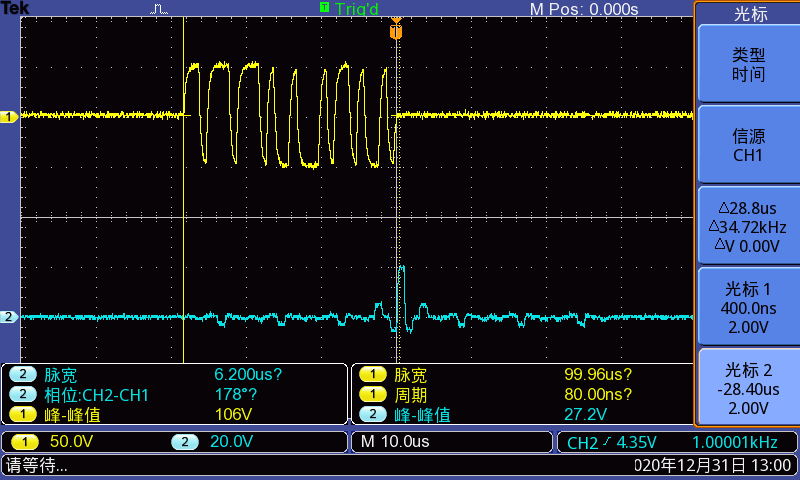
\includegraphics[
      width = \linewidth,
    ]{images/barker32.png}
    \caption{32 位互补码}%
    \label{fig:barker32}
  \end{subfigure}
  \caption{匹配滤波器}%
  \label{fig:mf}
\end{figure}

\begin{figure}[htbp]
  \centering
  \begin{subfigure}[htbp]{0.25\linewidth}
    \centering
    \includegraphics[
      width = \linewidth,
    ]{figures/rect.pdf}
    \caption{矩形脉冲}%
    \label{fig:rect_}
  \end{subfigure}
  \quad
  \begin{subfigure}[htbp]{0.25\linewidth}
    \centering
    \includegraphics[
      width = \linewidth,
    ]{figures/rect-out.pdf}
    \caption{矩形脉冲匹配滤波输出波形}%
    \label{fig:rect-out_}
  \end{subfigure}

  \begin{subfigure}[htbp]{0.25\linewidth}
    \centering
    \includegraphics[
      width = \linewidth,
    ]{figures/mrect.pdf}
    \caption{矩形脉冲串}%
    \label{fig:mrect_}
  \end{subfigure}
  \quad
  \begin{subfigure}[htbp]{0.25\linewidth}
    \centering
    \includegraphics[
      width = \linewidth,
    ]{figures/mrect-out.pdf}
    \caption{矩形脉冲串匹配滤波输出波形}%
    \label{fig:mrect-out_}
  \end{subfigure}

  \begin{subfigure}[htbp]{0.25\linewidth}
    \centering
    \includegraphics[
      width = \linewidth,
    ]{figures/m.pdf}
    \caption{M 序列}%
    \label{fig:m_}
  \end{subfigure}
  \quad
  \begin{subfigure}[htbp]{0.25\linewidth}
    \centering
    \includegraphics[
      width = \linewidth,
    ]{figures/m-out.pdf}
    \caption{M 序列匹配滤波输出波形}%
    \label{fig:m-out_}
  \end{subfigure}

  \begin{subfigure}[htbp]{0.25\linewidth}
    \centering
    \includegraphics[
      width = \linewidth,
    ]{figures/pn.pdf}
    \caption{伪随机截断码序列}%
    \label{fig:pn_}
  \end{subfigure}
  \quad
  \begin{subfigure}[htbp]{0.25\linewidth}
    \centering
    \includegraphics[
      width = \linewidth,
    ]{figures/pn-out.pdf}
    \caption{伪随机截断码匹配滤波输出波形}%
    \label{fig:pn-out_}
  \end{subfigure}

  \begin{subfigure}[htbp]{0.25\linewidth}
    \centering
    \includegraphics[
      width = \linewidth,
    ]{figures/barker13.pdf}
    \caption{13 位巴克码}%
    \label{fig:barker13_}
  \end{subfigure}
  \quad
  \begin{subfigure}[htbp]{0.25\linewidth}
    \centering
    \includegraphics[
      width = \linewidth,
    ]{figures/barker13-out.pdf}
    \caption{13 位巴克码匹配滤波输出波形}%
    \label{fig:barker13-out_}
  \end{subfigure}

  \begin{subfigure}[htbp]{0.25\linewidth}
    \centering
    \includegraphics[
      width = \linewidth,
    ]{figures/barker4_7.pdf}
    \caption{4、7 位组合巴克码}%
    \label{fig:barker4_7_}
  \end{subfigure}
  \quad
  \begin{subfigure}[htbp]{0.25\linewidth}
    \centering
    \includegraphics[
      width = \linewidth,
    ]{figures/barker4_7-out.pdf}
    \caption{4、7 位组合巴克码匹配滤波输出波形}%
    \label{fig:barker4_7-out_}
  \end{subfigure}
  \caption{输入波形和匹配滤波输出波形}%
  \label{fig:mf_}
\end{figure}

\begin{table}[htbp]
  \centering
  \caption{匹配滤波器}%
  \label{tab:mf}
  \csvautobooktabular[respect percent]{tables/mf.csv}
\end{table}

\langCVfile[matlab][lst:mf][matlab]{figures/mf.m}{figures/mf.m}

\begin{Exercise}
  对实验中出现的现象进行分析说明。
\end{Exercise}

\begin{Answer}
  信号匹配滤波后脉宽为原信号的 2 倍。

  \begin{itemize}
    \item 矩形脉冲的匹配滤波响应为三角脉冲。
    \item 矩形脉冲串的匹配滤波响应为包络为三角形的三角脉冲串。
    \item m 序列的匹配滤波响应近似为伪随机码的匹配滤波响应的周期延拓。
    \item 伪随机截断码的匹配滤波响应为图钉型函数。
    \item 13 位巴克码的匹配滤波响应为图钉型函数。
    \item 4、7 位组合巴克码的匹配滤波响应为图钉型函数。
    \item 32 位互补码的匹配滤波响应为图钉型函数。
  \end{itemize}
\end{Answer}

\begin{Exercise}
  实验报告中完成思考题。
\end{Exercise}

\begin{Answer}
  见章节~\ref{sec:\arabic{chapter}thought}。
\end{Answer}

\section{实验思考}%
\label{sec:\arabic{chapter}thought}

\begin{Exercise}
  为什么脉冲压缩输出波形为方波而不是三角波?
\end{Exercise}

\begin{Answer}
  因为该系统采用数字信号处理代替脉冲匹配滤波器。
\end{Answer}

\begin{Exercise}
  主副瓣比的测量方法有哪些?
\end{Exercise}

\begin{Answer}
  通过示波器测量幅度最大的主瓣电压和幅度第二大的副瓣电压之比。
\end{Answer}

\begin{Exercise}
  31 位 PN 截断码(m 序列中截取一个周期)与 31 位 m 序列的脉冲压缩输出波形为
  何不一样?
\end{Exercise}

\begin{Answer}
  31 位伪随机截断不具备周期性,为 m 序列的一个截断。截断起点、终点不同,输出
     波形不同。
\end{Answer}

\end{document}
